\documentclass{article}

\def\npart {II}
\def\nyear {2017}
\def\nterm {Michaelmas}
\def\nlecturer{Dr C. Brookes}
\def\ncourse{Galois Theory}
\ifx \nauthor\undefined
  \def\nauthor{Bhavik Mehta}
\else
\fi

\author{Based on lectures by \nlecturer \\\small Notes taken by \nauthor}
\date{\nterm\ \nyear}
\title{Part \npart\ -- \ncourse}

\usepackage[utf8]{inputenc}
\usepackage{amsmath}
\usepackage{amsthm}
\usepackage{amssymb}
\usepackage{enumerate}
\usepackage{mathtools}
\usepackage{graphicx}
\usepackage[dvipsnames]{xcolor}
\usepackage{tikz}
\usepackage{wrapfig}
\usepackage{centernot}
\usepackage{float}
\usepackage{braket}
\usepackage[hypcap=true]{caption}
\usepackage{enumitem}
\usepackage[colorlinks=true, linkcolor=mblue]{hyperref}
\usepackage[nameinlink,noabbrev]{cleveref}
\usepackage{nameref}
\usepackage[margin=1.5in]{geometry}

% Theorems
\theoremstyle{definition}
\newtheorem*{aim}{Aim}
\newtheorem*{axiom}{Axiom}
\newtheorem*{claim}{Claim}
\newtheorem*{cor}{Corollary}
\newtheorem*{conjecture}{Conjecture}
\newtheorem*{defi}{Definition}
\newtheorem*{eg}{Example}
\newtheorem*{ex}{Exercise}
\newtheorem*{fact}{Fact}
\newtheorem*{law}{Law}
\newtheorem*{lemma}{Lemma}
\newtheorem*{notation}{Notation}
\newtheorem*{prop}{Proposition}
\newtheorem*{question}{Question}
\newtheorem*{rrule}{Rule}
\newtheorem*{thm}{Theorem}
\newtheorem*{assumption}{Assumption}

\newtheorem*{remark}{Remark}
\newtheorem*{warning}{Warning}
\newtheorem*{exercise}{Exercise}

% \newcommand{\nthmautorefname}{Theorem}

\newtheorem{nthm}{Theorem}[section]
\newtheorem{nlemma}[nthm]{Lemma}
\newtheorem{nprop}[nthm]{Proposition}
\newtheorem{ncor}[nthm]{Corollary}
\newtheorem{ndef}[nthm]{Definition}

% Special sets
\newcommand{\C}{\mathbb{C}}
\newcommand{\N}{\mathbb{N}}
\newcommand{\Q}{\mathbb{Q}}
\newcommand{\R}{\mathbb{R}}
\newcommand{\Z}{\mathbb{Z}}

\newcommand{\abs}[1]{\left\lvert #1\right\rvert}
\newcommand{\norm}[1]{\left\lVert #1\right\rVert}
\renewcommand{\vec}[1]{\boldsymbol{\mathbf{#1}}}

\let\Im\relax
\let\Re\relax

\DeclareMathOperator{\Im}{Im}
\DeclareMathOperator{\Re}{Re}
\DeclareMathOperator{\id}{id}

\definecolor{mblue}{rgb}{0., 0.05, 0.6}


% preamble
\setcounter{section}{-1}
% and here we go!

\begin{document}
\maketitle

\section{Introduction}
The primary motivation of this course is to study the solutions of polynomial equations in one variable to wander whether there is a formula involving roots, a solution by radicals.  Quadratics were typically studied in school, while the solution in radicals for cubics and quartics has been known for a long time and studied in particular in 1770 by Lagrange.

In 1799, Ruffini claimed that there were some quintics that can't be solved by radicals, that is, there is no general formula, but it took until 1824 before Abel used existing ideas about permutations to produce the first accepted proof of insolubility, before dying in 1829.  Galois' main contribution was in 1831, when he gave the first explanation as to why some polynomials are soluble by radicals and others are not. He made use of the group of permutations of the roots of a polynomial, and realised in particular the importance of \emph{normal} subgroups.

Galois' work was not known generally in his lifetime - it was only published by Liouville in 1846, who realised that it tied in well with the work of Cauchy on permutations. Galois had submitted his work for various competitions and for entry into the Ecole Polytechnique in Paris.  Unfortunately Galois died in a duel in 1832, leaving a six and a half page letter indicating his thoughts about the future development of his theory.

\subsection{Course overview}
Most of this course is Galois Theory, but presented in a more modern fashion- in terms of field extensions.
Recall from GRM that if $f(t)$ is an irreducible polynomial in $k[t]$ where $k$ is a field, then $k[t]/(f(t))$ is a field, where $(f(t))$ denotes the ideal of $k[t]$ generated by $f(t)$, and this new field contains $k$.  In this way, we can see the field $k[t]/(f(t))$ as a field extension of $k$.

% TODO: sort this out with sensible formatting
% Galois' papers have been studied by Peter Neumann:
% The math writings of Evariste Galois, European Math Soc
% Different books: I. Steward Galois Theory, (something) and Hall
% contains a historcal introduction and covers almost all the syllabus.
% Artin Galois Theory
% Van der Waerden Modern Algebra (covers a lot more than Galois theory)
% Lang Algebra (late editions are preferred, covers a lot of algebra)
% Kaplansky Fields and Rings

\paragraph{Prerequisites} Quite a lot of the Groups, Rings and Modules course, but no modules except in one place where it's useful to know the structure of finite abelian groups. The DPMMS website has a Galois Theory page with a long history of example sheets and notes, in particular see Tony Scholl's 2013-4 course page.
\clearpage

\section{Field Extensions}
\begin{ndef}\hypertarget{def:fieldExt}
    A \textbf{field extension} $K \leq L$ is the inclusion of a field $K$ into another field $L$ with the same $0$, $1$, and where the restriction of $+$ and $.$ (in L) to $K$ gives the $+$ and $.$ of $K$.
\end{ndef}

\begin{eg}
    \leavevmode
    \begin{enumerate}[(i)]
        \item $\Q \leq \R$
        \item $\R \leq \C$
        \item $\Q \leq \Q(\sqrt{2}) = \Set{\lambda + \mu \sqrt{2} | \lambda, \mu \in \Q}$
        \item $\Set{\lambda + \mu i | \lambda, \mu \in \Q} = \Q(i) \leq \C$
    \end{enumerate}
\end{eg}

Suppose $K \leq L$ is a \hyperlink{def:fieldExt}{field extension}. Then $L$ is a $K$-vector space using the addition from the field structure and scalar multiplcation given by the multiplication in the field $L$.

\begin{ndef}\hypertarget{def:degreeOfFieldExt}
    The \textbf{degree} of $L$ over $K$ is $\dim_K L$, the $K$-vector space dimension of $L$. This may not be finite. We typically denote this by $\abs{L:K}$.
    If $\abs{L:K} < \infty$, then the extension is \textbf{finite}, otherwise the extension is \textbf{infinite}.
\end{ndef}

\begin{eg}\leavevmode
    \begin{enumerate}[(i)]
        \item $\abs{\C:\R} = 2$, with $\R$-basis $1, i$
        \item $\abs{\Q(i):\Q} = 2$, with $\Q$-basis $1, i$
        \item $\Q \leq \R$ is an infinite extension.
    \end{enumerate}
\end{eg}

\begin{nthm}[\hypertarget{def:towerLaw}{Tower law}]
    Suppose $K \leq L \leq M$ are field extensions. Then $\abs{M:K}$ = $\abs{M:L}\abs{L:K}$.
\end{nthm}
\begin{proof}
    Assume that $\abs{M:L} < \infty$, and $\abs{L:K} < \infty$.
    Take an $L$-basis of $M$, given by $\Set{f_1, \dotsc, f_b}$, and a $K$-basis of $L$ given by $\Set{e_1, \dotsc, e_a}$.
    Take $m \in M$, so $m = \sum_{i=1}^b \mu_i f_i$ for some $\mu_i \in L$.
    Similarly, $\mu_i = \sum_{j=1}^a \lambda_{ij} e_j$ for some $\lambda_{ij} \in K$, so

    \begin{equation*}
        m = \sum_{i=1}^b \sum_{j=1}^a \lambda_{ij} e_j f_i
    \end{equation*}
    Thus $\Set{e_j f_i | 1 \leq j \leq a, 1 \leq i \leq a}$ span $M$.

    Linear independence:
    It's enough to show that if $0 = m = \sum \sum \lambda_{ij} e_j f_i$ then $\lambda_{ij}$ are all zero.
    However if $m = 0$ the linear independence of $f_i$ forces each $\mu_i = 0$.
    Then the linear indepedence of $e_j$ forces $\lambda_{ij}$ all to be zero, as required.
\end{proof}

The tower law will not be proved for \hyperlink{def:degreeOfFieldExt}{infinite} extensions, but observe that if $M$ is an infinite extension of $L$ then it is an infinite extension of $K$, and similarly if $L$ is an infinite extension of $K$ then the larger field $M$ must also be an infinite extension of $K$.

\subsection{Motivatory Example}
Observe $\Q \leq \Q\left(\sqrt{2}\right) \leq \Q\left(\sqrt{2}, i\right)$
\begin{enumerate}[(i)]
    \item $\Q\left(\sqrt{2}\right)$ has basis $1, \sqrt{2}$ over $\Q$.
    \item $\Q\left(\sqrt{2}, i\right)$ has basis $1, i$ as a $\Q\left(\sqrt{2}\right)$--vector space.
    \item $\Q\left(\sqrt{2}, i\right)$ has basis $1, \sqrt{2}, i, i\sqrt{2}$ over $\Q$.
\end{enumerate}
\begin{equation*}
    \abs{\Q\left(i, \sqrt{2}\right):\Q} = 4 = 2 \cdot 2 = \abs{\Q\left(i, \sqrt{2}\right) : \Q\left(\sqrt{2}\right)} \abs{\Q\left(\sqrt{2}\right):\Q}
\end{equation*}

Any intermediate field strictly between $\Q$ and $\Q\left(\sqrt{2}, i\right)$ must be of degree $2$ by the tower law.
What are these intermediate fields? There are $\Q\left(\sqrt{2}\right)$, $\Q(i)$ and $\Q\left(i\sqrt{2}\right)$, but are these all?

The Galois correspodence arising in the Fundamental Theorem of Galois theory gives an order reversing bijection between the lattice of intermediate subfields and the subgroups of a group of ring automorphisms of the big field (in this case $\Q\left(i, \sqrt{2}\right)$) that fix the smaller field elementwise.
For instance, consider the ring automorphisms of $\Q\left(i, \sqrt{2}\right)$ that fix $\Q$:
\begin{align*}
    e : \sqrt{2} &\mapsto \sqrt{2} \\
               i &\mapsto i \\
    g : \sqrt{2} &\mapsto \sqrt{2} \\
               i &\mapsto -i \\
    h : \sqrt{2} &\mapsto -\sqrt{2} \\
               i &\mapsto i \\
    gh: \sqrt{2} &\mapsto -\sqrt{2} \\
               i &\mapsto -i
\end{align*}
Notice that $i$ and $-i$ play the same role in the field $\Q\left(\sqrt{2}, i\right)$, both roots of $t^2 + 1 = 0$, similarly $\sqrt{2}$ and $-\sqrt{2}$ are both roots of $t^2 - 2 = 0$.  The automorphism $e$ is seen to be identity, and $g$ is conjugation.
These four form the group of order $4 = \abs{\Q\left(\sqrt{2}, i\right) : \Q}$.

\begin{center}
    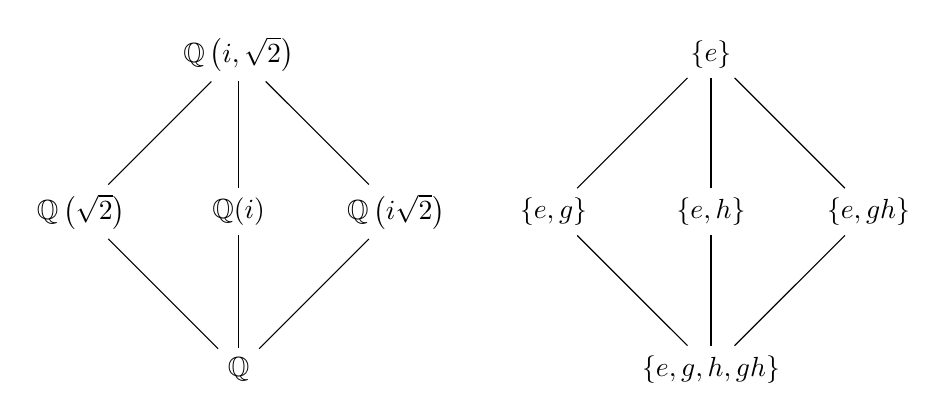
\begin{tikzpicture}[node distance=2cm]
        \node (Q)                  {$\mathbb{Q}$};
        \node (Qi)  [above of=Q]   {$\mathbb{Q}(i)$};
        \node (Qi2) [right of=Qi]  {$\mathbb{Q}\left(i\sqrt{2}\right)$};
        \node (Q2)  [left of=Qi]   {$\mathbb{Q}\left(\sqrt{2}\right)$};
        \node (Q2i) [above of=Qi]  {$\mathbb{Q}\left(i, \sqrt{2}\right)$};
        \node (eg)  [right of=Qi2] {$\{e, g\}$};
        \node (egh) [right of=eg]  {$\{e, h\}$};
        \node (eh)  [right of=egh] {$\{e, gh\}$};
        \node (G)   [below of=egh] {$\{e, g, h, gh\}$};
        \node (e)   [above of=egh] {$\{e\}$};
        \draw (Q)   -- (Qi2);
        \draw (Q)   -- (Q2);
        \draw (Q)   -- (Qi);
        \draw (Qi2) -- (Q2i);
        \draw (Q2)  -- (Q2i);
        \draw (Qi)  -- (Q2i);
        \draw (G)   -- (eg);
        \draw (G)   -- (egh);
        \draw (G)   -- (eh);
        \draw (eg)  -- (e);
        \draw (egh) -- (e);
        \draw (eh)  -- (e);
    \end{tikzpicture}
\end{center}

The recipe for producing an intermediate subfield from a subgroup is to take the elements of $\Q\left(i, \sqrt{2}\right)$ which are fixed by all elements of the subgroup.
For instance, $\Q\left(i \sqrt{2}\right)$ is the field of elements fixed by both $e$ and $gh$.

This correspondence doesn't always work for all finite field extensions.  It works for Galois extensions.
In the correspondence, normal extensions correspond to normal subgroups.
In this example, all subgroups are normal and the extensions are normal.
We'll also prove the Primitive Element Theorem, which in the context of finite extensions of $\Q$ tells us that they are necessarily of the form $\Q(\alpha)$ for some $\alpha$, for instance $\Q(i, \sqrt{2}) = \Q(i + \sqrt{2})$.

\subsection{Review of GRM}
\begin{ndef}\hypertarget{def:algebraic}
    Suppose $K \leq L$ is a field extension. Take $\alpha \in L$ and define
    \begin{equation*}
        I_\alpha = \set{f \in K(t) | f(\alpha) = 0}
    \end{equation*}
    We say $\alpha$ is \textbf{algebraic} over $K$ if $I_\alpha \ne 0$.  Otherwise $\alpha$ is \textbf{transcendental}.
    We say $L$ is algebraic over $K$ if $\alpha$ is algebraic over $K$ for all $\alpha \in L$.
\end{ndef}

\begin{remark}
    We can see $I_\alpha$ is an ideal of $K[t]$ since it is the kernel of the ring homomorphism $K[t] \to L$ given by $f(t) \mapsto f(\alpha)$.
\end{remark}

\begin{eg}
    \leavevmode
    \begin{enumerate}[(i)]
        \item $\sqrt{2}$ is \hyperlink{def:algebraic}{algebraic} over $\Q$
        \item $\pi$ is algebraic over $\Q$
    \end{enumerate}
\end{eg}

\begin{nlemma}
    Let $K \leq L$ be a \hyperlink{def:degreeOfFieldExt}{finite} \hyperlink{def:fieldExt}{field extension}. Then $L$ is \hyperlink{def:algebraic}{algebraic} over $K$.
\end{nlemma}

\begin{proof}
    Let $\abs{L:K}=n$, and take $\alpha \in L$. Consider $1, \alpha, \alpha^2, \dotsc, \alpha^n$, which must be linearly dependent in the $n$-dimensional $K$--vector space $L$.
    So, $\sum_{i=0}^n \lambda_i \alpha^i = 0$ for some $\lambda \in K$ not all zero, and hence $\alpha$ is a root of $f(t) = \sum_{i=0}^n \lambda_i t^i$, so $\alpha$ is \hyperlink{def:algebraic}{algebraic} over $K$.
    $\alpha$ was arbitrary, so $L$ is algebraic over $K$.
\end{proof}

\begin{ndef}\hypertarget{def:minimalPoly}
    The non-zero ideal $I_\alpha$ (where $\alpha$ is \hyperlink{def:algebraic}{algebraic} over $K$) is principal since $K[t]$ is a principal ideal domain.
    In particular, we can say $I_\alpha = (f_\alpha(t))$ where $f_\alpha(t)$ can be assumed to be monic.
    Such a monic $f_\alpha(t)$ is the \textbf{minimal polynomial} of $\alpha$ over $K$.
\end{ndef}

\begin{remark}
    Multiplication by $\alpha$ within the field $L$ gives a $K$--linear map $L \to L$, an automorphism (if $\alpha \ne 0$).  In GRM, we have seen the \hyperlink{def:minimalPoly}{minimal polynomial} of a linear map is unique.
\end{remark}

\begin{eg}\leavevmode
    \begin{enumerate}[(1)]
        \item The minimal polynomial of $\sqrt{2}$ over $\Q$ is $t^2 - 2$.
        \item The minimal polynomial of $\sqrt{2}$ over $\R$ is $t - \sqrt{2}$.
    \end{enumerate}
\end{eg}

\begin{nlemma}
    Suppose $K \leq L$ is a \hyperlink{def:fieldExt}{field extension}, $\alpha \in L$ and $\alpha$ is \hyperlink{def:algebraic} over $K$.
    Then the \hyperlink{def:minimalPoly}{minimal polynomial} $f_\alpha(t)$ of $\alpha$ over $K$ is irreducible in $K[t]$ and $I_\alpha$ is a prime ideal.
\end{nlemma}

\begin{proof}
    Suppose $f_\alpha(t) = p(t) q(t)$. We aim to show $p(t)$ or $q(t)$ is a unit in $K[t]$.
    But $0 = f_\alpha(\alpha) = p(\alpha) q(\alpha)$, so $p(\alpha) = 0$ or $q(\alpha) = 0$, without loss of generality take $p(\alpha) = 0$, thus $p(t) \in I_\alpha$.
    But $I_\alpha=(f_\alpha(t))$, so $p(t) = f_\alpha(t) r(t)$, giving $f_\alpha(t) = f_\alpha(t) r(t) q(t)$ and so $r(t) q(t) = 1$ in $K[t]$, and $q(t)$ is a unit, as required.
    Recall from GRM that irreducible elements of $K[t]$ are prime and hence generate prime ideals of $K[t]$. So $I_\alpha$ is a prime ideal.
\end{proof}

\begin{ndef}\hypertarget{def:genField}
    Suppose $K\leq L$ is a \hyperlink{def:fieldExt}{field extension} and $\alpha \in L$.  $K(\alpha)$ is defined to be the smallest subfield of $L$ containing $K$ and $\alpha$.
    It's called the field \textbf{generated} by $K$ and $\alpha$.  We say that $L$ is a \textbf{simple extension} if $L = K(\beta)$ for some $\beta \in L$.
\end{ndef}
\end{document}
